% !TEX root = ./Vortrag.tex
\begin{frame}[label=title]{}
\titlepage
\begin{center} Betreuer: Benjamin Reh \& Thomas Kloepfer
\end{center}
\end{frame}
\begin{frame}[label=title]{}
\tableofcontents
\end{frame}

\section{Projektziel}
\begin{frame}{Projektziel}
\begin{exampleblock}{Zielvorgaben}
\begin{itemize}
\item Roboterarm mit zwei Gelenken
\item zugehöriges Xylophon
\end{itemize}
\end{exampleblock}
\\[0.5cm]
\begin{exampleblock}{Umsetzung}
\begin{itemize}
\item halbkreisförmiges Xylophon
\item Microcontroller gesteuerter Servoarm mit Schlägel
\item Steuerung über serielle Schnittstelle mit einem Terminalprogramm
\end{itemize}
\end{exampleblock}
\end{frame}

% Local background must be enclosed by curly braces for grouping.
{
\usebackgroundtemplate{\includegraphics[trim=0cm 0cm -10cm -10cm,clip=true,height=1.25\paperheight,angle=90]{Plots/Robo1.jpg}}%
\begin{frame}{Komponenten}
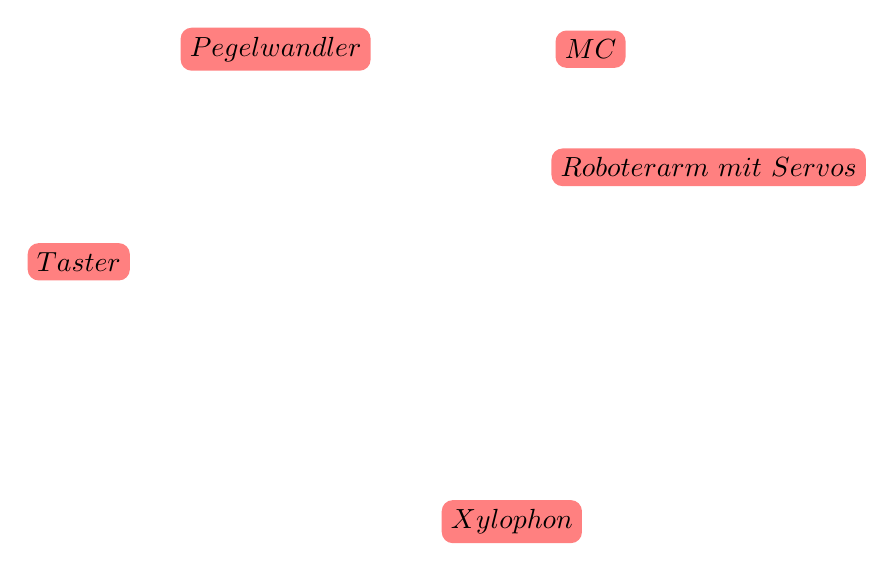
\begin{tikzpicture}
	\node (MC) at (8,1) [rounded corners=4pt, fill=red!50] {$MC$};
	\node (Servo) at (9.5,-0.5) [rounded corners=4pt, fill=red!50] {$Roboterarm\ mit\ Servos$};
	\node (Pegelwandler) at (4,1) [rounded corners=4pt, fill=red!50] {$Pegelwandler$};
	\node (A) at (7,-5) [rounded corners=4pt, fill=red!50] {$Xylophon$};
	\node (B) at (1.5,-1.7) [rounded corners=4pt, fill=red!50] {$Taster$};
\end{tikzpicture}
\end{frame}}

\section{Aufbau des Roboters}

\begin{frame}{Aufbau des Roboters}
\begin{itemize}
\item Löten des MC
\item Aufbau des Schlage Mechanismus
\item Konstruktion des Roboterarms
\item Programmierung des MC
\item Aufabu des Xylophons
\item Programmierung des Konsolen Programms
\item Fehlerbehebung/Verbesserungen
\end{itemize}
\end{frame}

\section{Funktionen}
\begin{frame}{Funktionen}
\begin{exampleblock}{Betrieb mit PC}
\begin{itemize}
\item Manueller Modus
\item Lied Modus
\item neues Lied überspielen
\end{itemize}
\end{exampleblock}
\\[0.5cm]
\begin{exampleblock}{Betrieb ohne PC}
\begin{itemize}
\item gespeichertes Lied starten mit Taster
\end{itemize}
\end{exampleblock}
\end{frame}

\section{Programmstruktur}
{
\usebackgroundtemplate{\includegraphics[trim=31cm 45cm -1cm 0cm, clip=true,angle=90,width=\textwidth]{Plots/Diagramm11.pdf}}%
\begin{frame}{Programmstruktur}
\end{frame}}


\begin{frame}[containsverbatim]{Lied vorbereiten}
\begin{columns}
\column{0.49\paperwidth}
\vspace{-1cm}
\begin{lstlisting}
typedef union
{
	struct 
	{
		uint16_t tonpos_ii;
		uint16_t tonlaenge_i;
	} daten;
	
	struct 
	{
		uint16_t tonpos_i;
		uint16_t liedlaenge;
	} daten2;
	
	char inhalt[4];
}packet;
\end{lstlisting}
\column{0.49\paperwidth}
\vspace{-0.5cm}
\begin{figure}
\center
\includegraphics[trim=4cm 3cm 5cm 8cm, clip=true,height=\textheight]{Plots/Diagramm2.pdf}
\end{figure}
\end{columns}
\end{frame}

\begin{frame}[containsverbatim]{Lied übertragen}
\begin{columns}
\column{0.5\paperwidth}
\begin{lstlisting}[tabsize=2]
void play(int offset) {	

union packet p;
while(1)
{
	int i;
	for(i=0; i<4; i++)
	{
		p.inhalt[i]=uart_getc();
	}
	if(p.daten.tonpos_ii==0)
	{
		schlage();
		uart_putc('f');
		break;
	}
	schlage();
	setServo(1,p.daten.tonpos_ii+offset);
	_delay_ms(p.daten.tonlaenge_i-schld);
	uart_putc('r');
}
\end{lstlisting}
\column{0.5\paperwidth}
\vspace{-0.5cm}
\begin{figure}
\center
\includegraphics[trim=6.8cm 53cm 27.8cm 7.5cm, clip=true,width=\textwidth,height=0.8\textheight]{Plots/Diagramm3.pdf}
\end{figure}
\end{columns}
\end{frame}

\begin{frame}{Manuelles Spiel}
\begin{columns}
\column{0.5\paperwidth}
\vspace{-1cm}
\begin{exampleblock}{Manuelles Spiel}
\begin{itemize}
\item MC initialisiert mit "m"
\item Eingabe eines Tons über die Tastatur
\item Übertragen der Tonposition mit fester Tonlänge
\item Beenden des manuellen Spiels durch Eingabe einer Zahl
\item MC sendet "f"\ und geht in Ausgangsposition zurück
\end{itemize}
\end{exampleblock}
\column{0.5\paperwidth}
\begin{figure}
\center
\includegraphics[trim=11cm 18cm 10cm 29cm, clip=true,angle=90, clip=true,height=\textheight]{Plots/Diagramm1.pdf}
\end{figure}
\end{columns}
\end{frame}


\begin{frame}[containsverbatim]{Neues Lied übertragen}
%\vspace{-1cm}
\begin{exampleblock}{Neues Lied übertragen}
\begin{itemize}
\item MC initialisiert mit "n"
\item Eingabe eines Liedes wie beim Liedmodus
\item Übertragen des Liedes wie beim Liedmodus
\item Aber: Speichern des Liedes als Array im EEPROM Speicher des MC
\item Lied abrufbar durch Drücken des Tasters
\end{itemize}
\end{exampleblock}
\begin{lstlisting}[tabsize=2, basicstyle=\ttfamily\scriptsize]
eeprom_read_block (tondauer, tonlaengen, sizeof(tonlaengen));
eeprom_read_block (tonpos, tonpositionen, sizeof(tonpositionen));
	
else if (s=='n')
{
	eeprom_write_block (tondauer, tonlaengen,sizeof(tondauer));
	eeprom_write_block (tonpos, tonpositionen,sizeof(tonpos));
	uart_putc('f');
}
\end{lstlisting}
\end{frame}

\begin{frame}{GUI}
\begin{itemize}
\item Grafische Benutzeroberfläche
\item erstellt mit wxGlade
\item basierend auf wxWidgets
\end{itemize}
\begin{figure}
\center
\includegraphics[trim=0cm 0cm 0cm 0cm, clip=true,width=\textwidth]{Plots/GUI.pdf}
\end{figure}
\end{frame}

\begin{frame}[containsverbatim]{GNU Gettext}
\begin{itemize}
\item Internationalisierung des Programms ohne Kenntnis des Quellcodes
\item Übersetzung in extra Datei
\item bis jetzt 2 Sprachen vor dem Start wählbar (DE,EN)
\end{itemize}
{\scriptsize http://www.gnu.org/software/gettext/}
\begin{exampleblock}{Code}
\begin{lstlisting}
printf("Ein wenig Text");

printf(gettext("Ein wenig Text"));
\end{lstlisting}
\end{exampleblock}
\end{frame}

\section{Probleme}

\begin{frame}{Probleme}
\begin{itemize}
\item Schlägel
\item Spannung
\item zu kräftiger Servo
\item defekter Pegelwandler
\end{itemize}
\end{frame}

\section{Ausblick}

\begin{frame}{Ausblick}
\begin{itemize}
\item Zusammenspiel mit Flötenroboter u.ä.
\item Verbesserung des manuellen Modus
\item Einbinden von MIDI Dateien
\item Verbesserung GUI
\end{itemize}
\end{frame}

\section{Vorführung}
\setbeamercolor{background canvas}{bg=black}
\begin{frame}[plain]

\end{frame}
